\documentclass[11pt]{article}
\usepackage[textwidth=18.0cm, textheight=23.0cm, top=2.0cm]{geometry}
\usepackage{pst-all}
\usepackage{amssymb}
\usepackage{tikz}
\usepackage{underscore}\begin{document}
\pagestyle{empty}


ClassName: \underline{\textbf{Class_07.2bp-13}}
\par
BinSize: \underline{\textbf{100 × 100}}
\par
ReduceSize: \underline{\textbf{100 × 100}}
\par
TypeNum: \underline{\textbf{39}}
\par
Num: \underline{\textbf{40}}
\par
OutS: \underline{\textbf{140000}}
\par
InS: \underline{\textbf{111847}}
\par
Rate: \underline{\textbf{0.799}}
\par
UB: \underline{\textbf{14}}
\par
LB0: \underline{\textbf{14}}
\par
LB: \underline{\textbf{14}}
\par
LBWithCut: \underline{\textbf{14}}
\par
NodeCut: \underline{\textbf{0}}
\par
ExtendedNodeCnt: \underline{\textbf{1}}
\par
GenNodeCnt: \underline{\textbf{1}}
\par
PrimalNode: \underline{\textbf{0}}
\par
ColumnCount: \underline{\textbf{14}}
\par
TotalCutCount: \underline{\textbf{0}}
\par
RootCutCount: \underline{\textbf{0}}
\par
LPSolverCnt: \underline{\textbf{1}}
\par
PricingSolverCnt: \underline{\textbf{0}}
\par
BranchAndBoundNum: \underline{\textbf{1}}
\par
isOpt: \underline{\textbf{true}}
\par
TimeOnInitSolution: \underline{\textbf{0.110 s}}
\par
TimeOnPrimal: \underline{\textbf{0.000 s}}
\par
TimeOnPricing: \underline{\textbf{0.000 s}}
\par
TimeOnRmp: \underline{\textbf{0.063 s}}
\par
TotalTime: \underline{\textbf{0.235 s}}
\par
\newpage



\begin{tikzpicture}[shorten >=1pt,scale=1.0,every node/.style={scale=1.0},->]
\tikzstyle{vertex}=[circle,fill=black!25,minimum size=14pt,inner sep=0pt]
\filldraw[fill=gray!40!white, draw=black] (0,0) rectangle (15.0,15.0);
\foreach \name/\x/\y/\w/\h in {99x97/0.0/0.0/14.85/14.549999999999999}
\filldraw[fill=white!40!white, draw=black] (\x,\y) rectangle node[draw] (\name) {\name} ++(\w,\h);
\end{tikzpicture}


w =99 , h =97 , x =0 , y =0 , v =9603
\par
\newpage


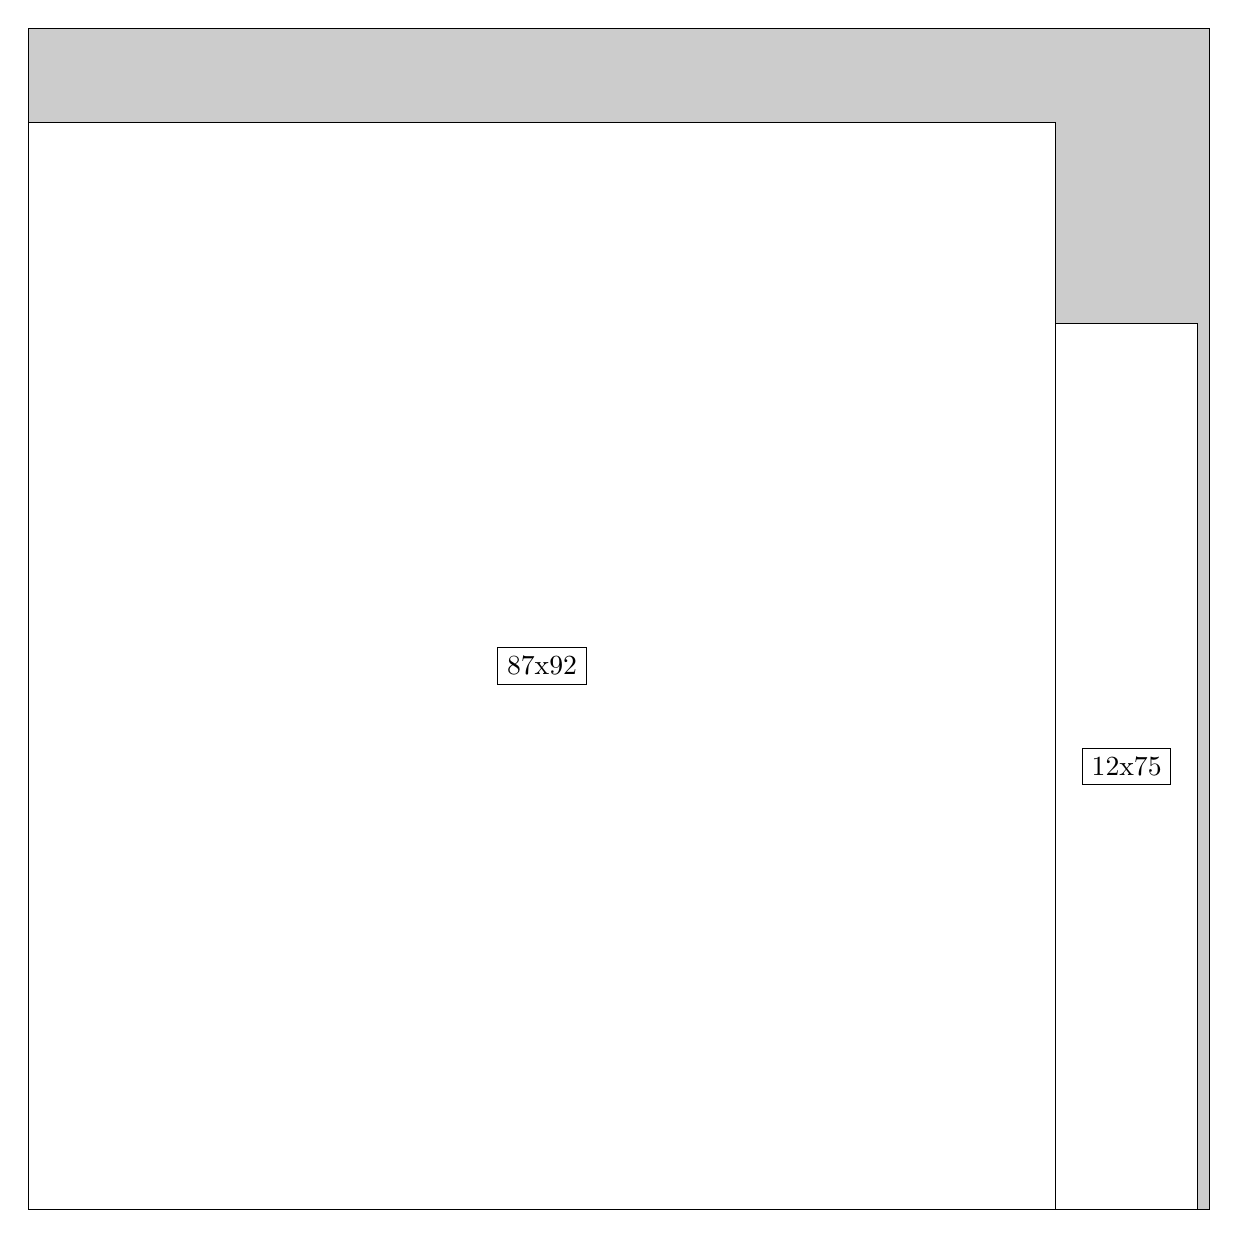
\begin{tikzpicture}[shorten >=1pt,scale=1.0,every node/.style={scale=1.0},->]
\tikzstyle{vertex}=[circle,fill=black!25,minimum size=14pt,inner sep=0pt]
\filldraw[fill=gray!40!white, draw=black] (0,0) rectangle (15.0,15.0);
\foreach \name/\x/\y/\w/\h in {87x92/0.0/0.0/13.049999999999999/13.799999999999999,12x75/13.049999999999999/0.0/1.7999999999999998/11.25}
\filldraw[fill=white!40!white, draw=black] (\x,\y) rectangle node[draw] (\name) {\name} ++(\w,\h);
\end{tikzpicture}


w =87 , h =92 , x =0 , y =0 , v =8004
\par
w =12 , h =75 , x =87 , y =0 , v =900
\par
\newpage


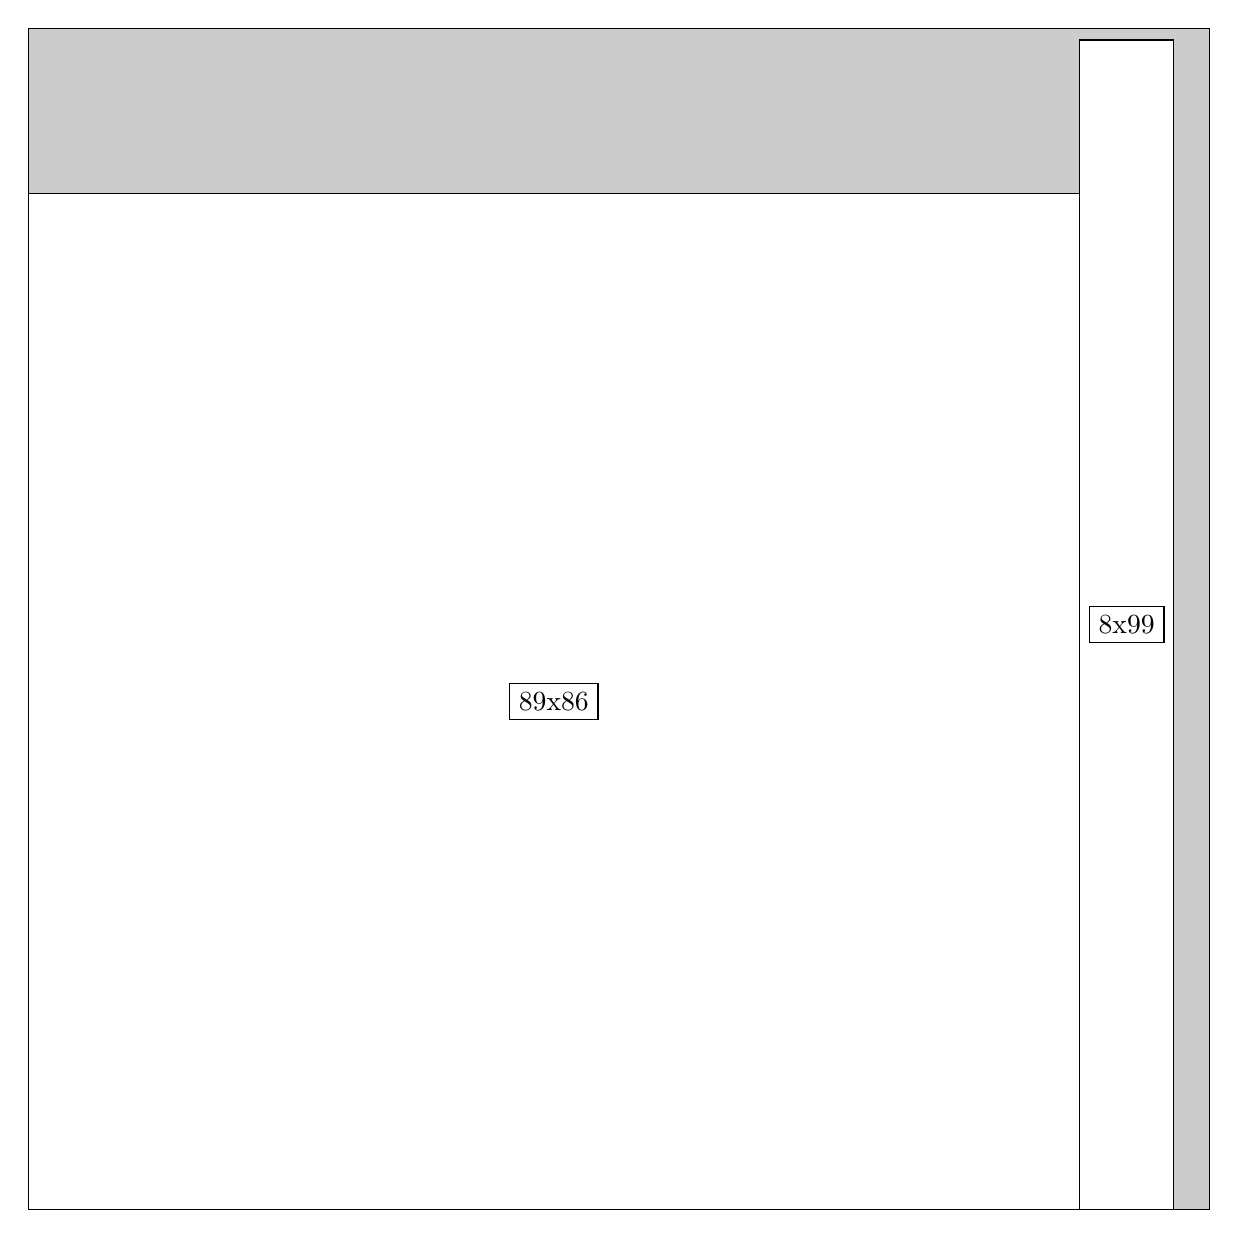
\begin{tikzpicture}[shorten >=1pt,scale=1.0,every node/.style={scale=1.0},->]
\tikzstyle{vertex}=[circle,fill=black!25,minimum size=14pt,inner sep=0pt]
\filldraw[fill=gray!40!white, draw=black] (0,0) rectangle (15.0,15.0);
\foreach \name/\x/\y/\w/\h in {89x86/0.0/0.0/13.35/12.9,8x99/13.35/0.0/1.2/14.85}
\filldraw[fill=white!40!white, draw=black] (\x,\y) rectangle node[draw] (\name) {\name} ++(\w,\h);
\end{tikzpicture}


w =89 , h =86 , x =0 , y =0 , v =7654
\par
w =8 , h =99 , x =89 , y =0 , v =792
\par
\newpage


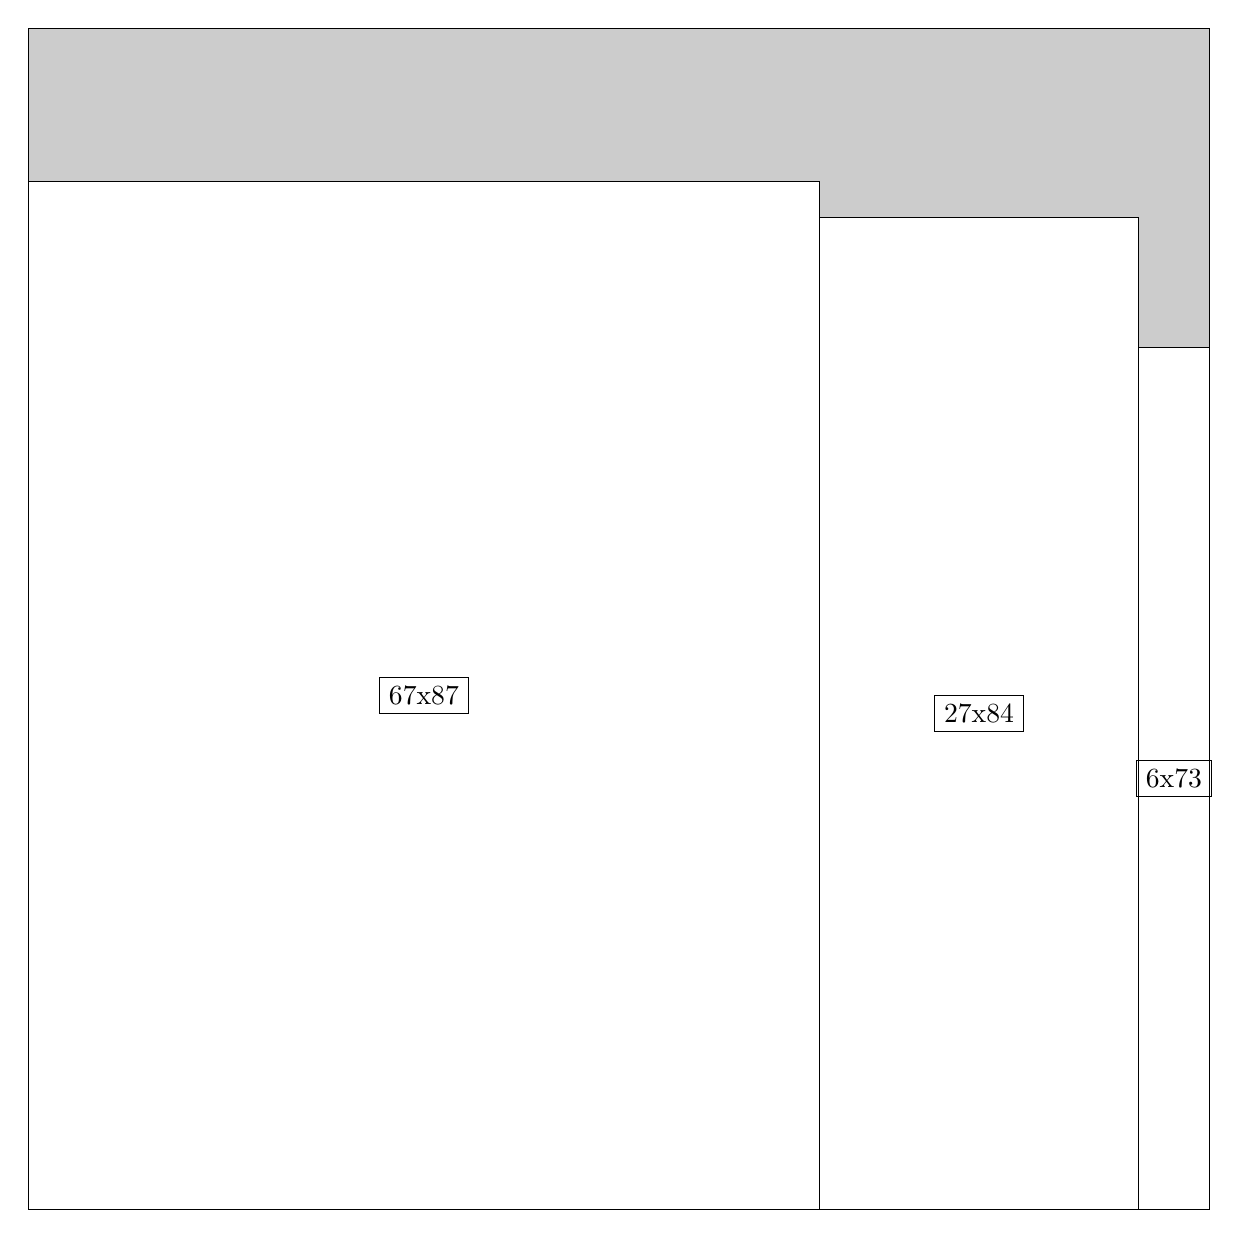
\begin{tikzpicture}[shorten >=1pt,scale=1.0,every node/.style={scale=1.0},->]
\tikzstyle{vertex}=[circle,fill=black!25,minimum size=14pt,inner sep=0pt]
\filldraw[fill=gray!40!white, draw=black] (0,0) rectangle (15.0,15.0);
\foreach \name/\x/\y/\w/\h in {67x87/0.0/0.0/10.049999999999999/13.049999999999999,27x84/10.049999999999999/0.0/4.05/12.6,6x73/14.1/0.0/0.8999999999999999/10.95}
\filldraw[fill=white!40!white, draw=black] (\x,\y) rectangle node[draw] (\name) {\name} ++(\w,\h);
\end{tikzpicture}


w =67 , h =87 , x =0 , y =0 , v =5829
\par
w =27 , h =84 , x =67 , y =0 , v =2268
\par
w =6 , h =73 , x =94 , y =0 , v =438
\par
\newpage


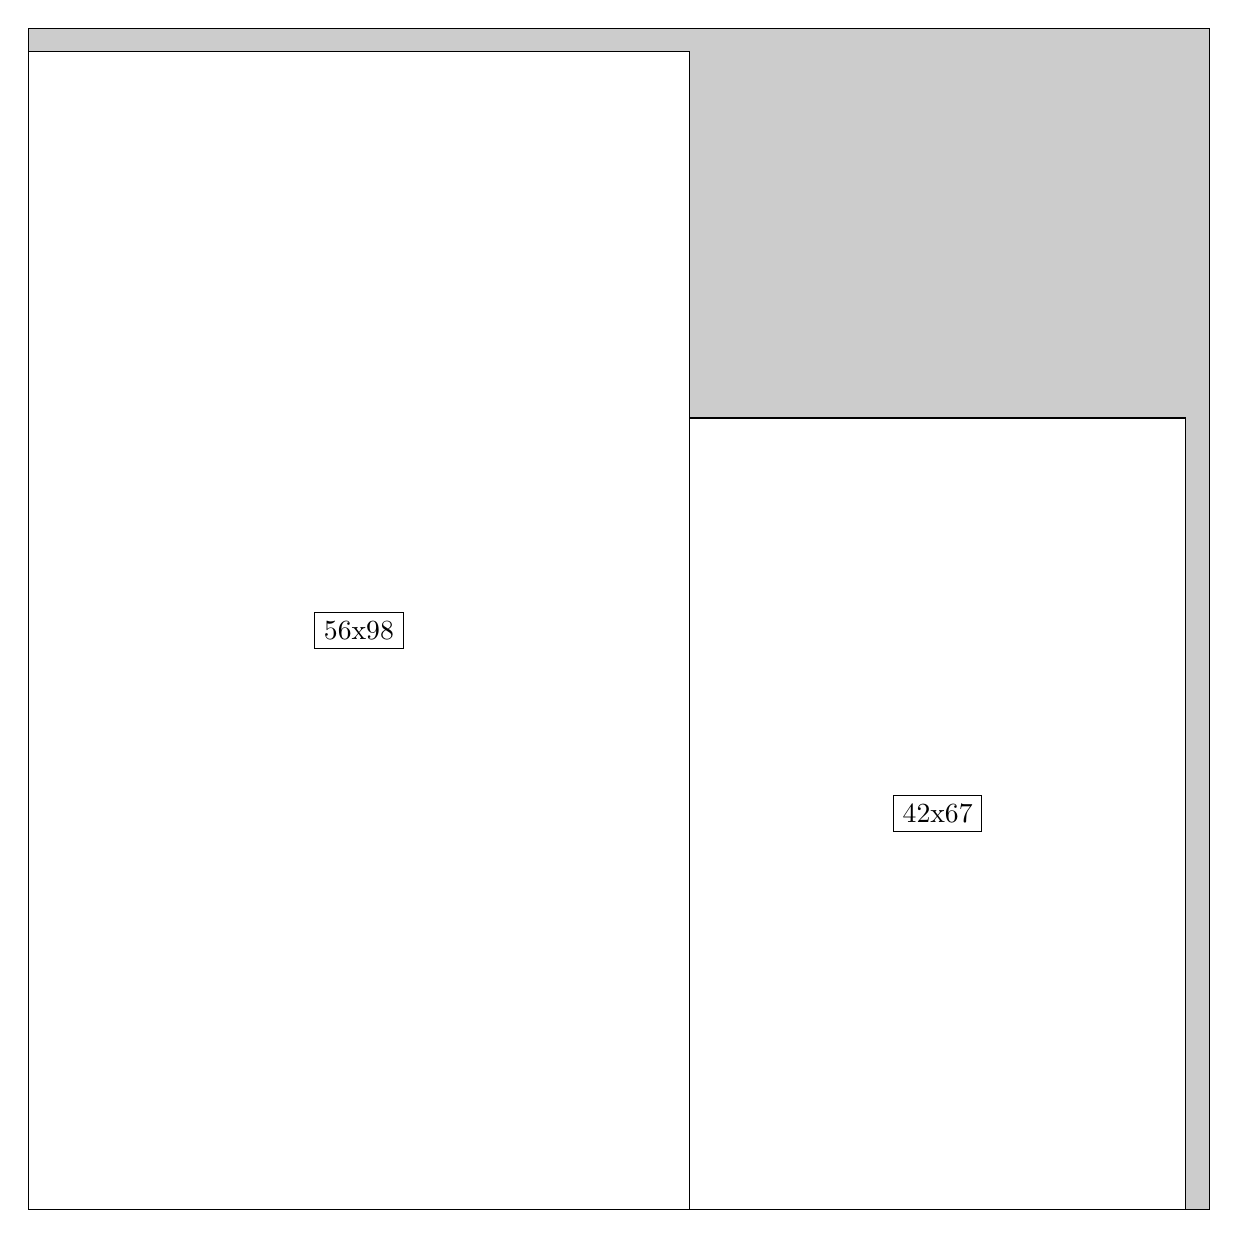
\begin{tikzpicture}[shorten >=1pt,scale=1.0,every node/.style={scale=1.0},->]
\tikzstyle{vertex}=[circle,fill=black!25,minimum size=14pt,inner sep=0pt]
\filldraw[fill=gray!40!white, draw=black] (0,0) rectangle (15.0,15.0);
\foreach \name/\x/\y/\w/\h in {56x98/0.0/0.0/8.4/14.7,42x67/8.4/0.0/6.3/10.049999999999999}
\filldraw[fill=white!40!white, draw=black] (\x,\y) rectangle node[draw] (\name) {\name} ++(\w,\h);
\end{tikzpicture}


w =56 , h =98 , x =0 , y =0 , v =5488
\par
w =42 , h =67 , x =56 , y =0 , v =2814
\par
\newpage


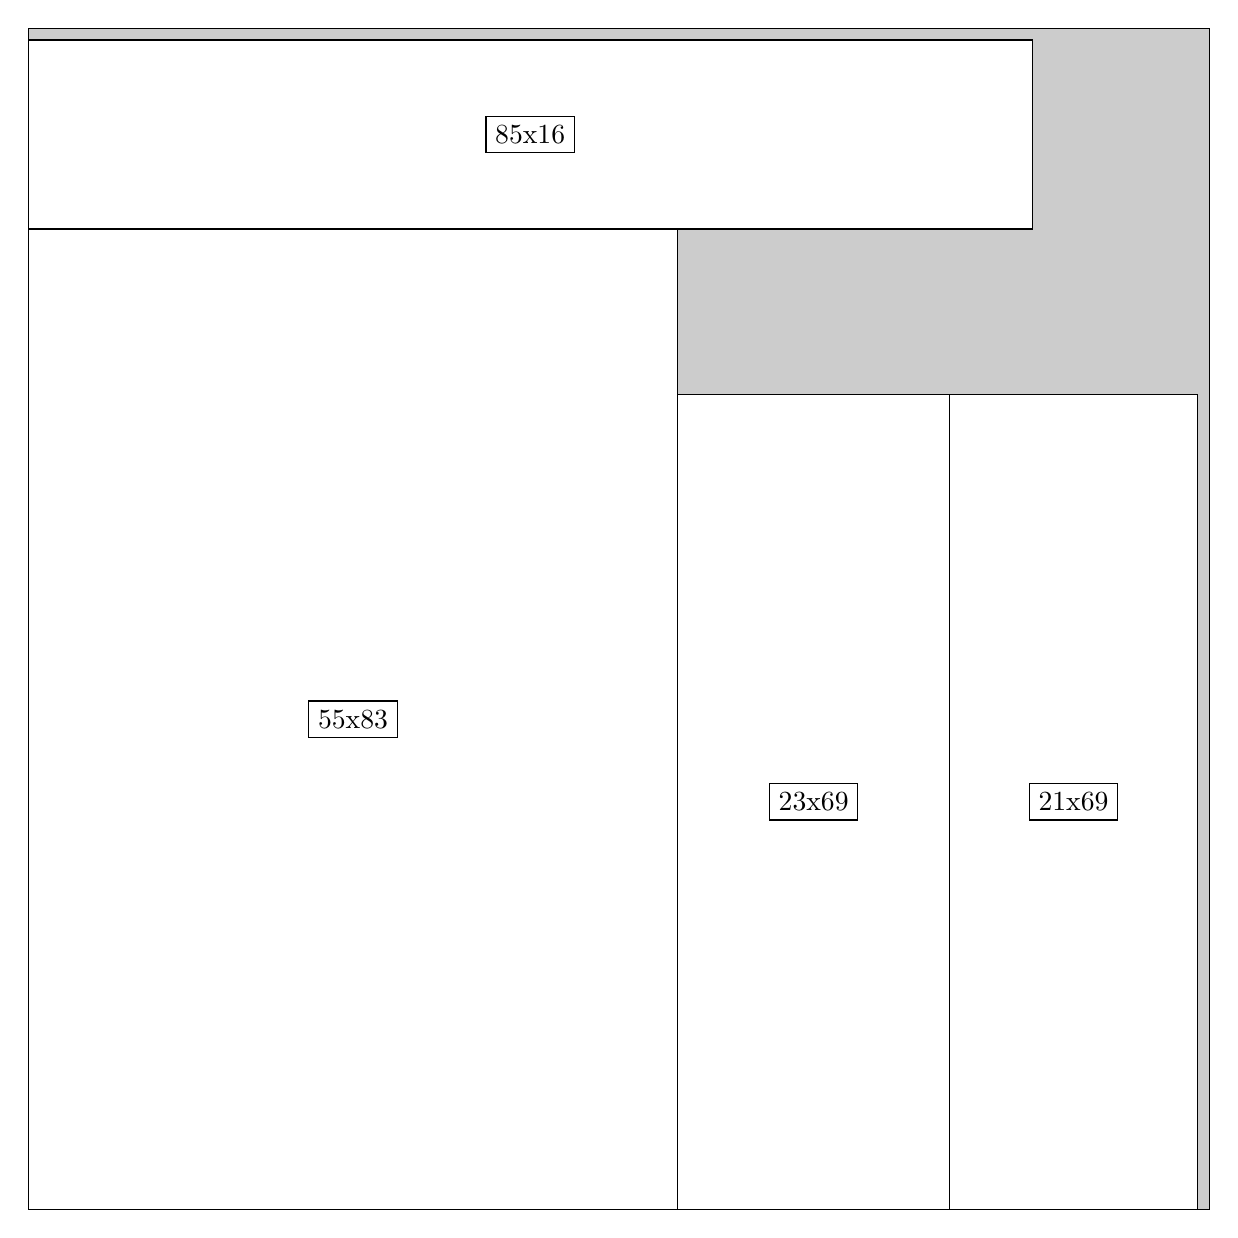
\begin{tikzpicture}[shorten >=1pt,scale=1.0,every node/.style={scale=1.0},->]
\tikzstyle{vertex}=[circle,fill=black!25,minimum size=14pt,inner sep=0pt]
\filldraw[fill=gray!40!white, draw=black] (0,0) rectangle (15.0,15.0);
\foreach \name/\x/\y/\w/\h in {55x83/0.0/0.0/8.25/12.45,23x69/8.25/0.0/3.4499999999999997/10.35,21x69/11.7/0.0/3.15/10.35,85x16/0.0/12.45/12.75/2.4}
\filldraw[fill=white!40!white, draw=black] (\x,\y) rectangle node[draw] (\name) {\name} ++(\w,\h);
\end{tikzpicture}


w =55 , h =83 , x =0 , y =0 , v =4565
\par
w =23 , h =69 , x =55 , y =0 , v =1587
\par
w =21 , h =69 , x =78 , y =0 , v =1449
\par
w =85 , h =16 , x =0 , y =83 , v =1360
\par
\newpage


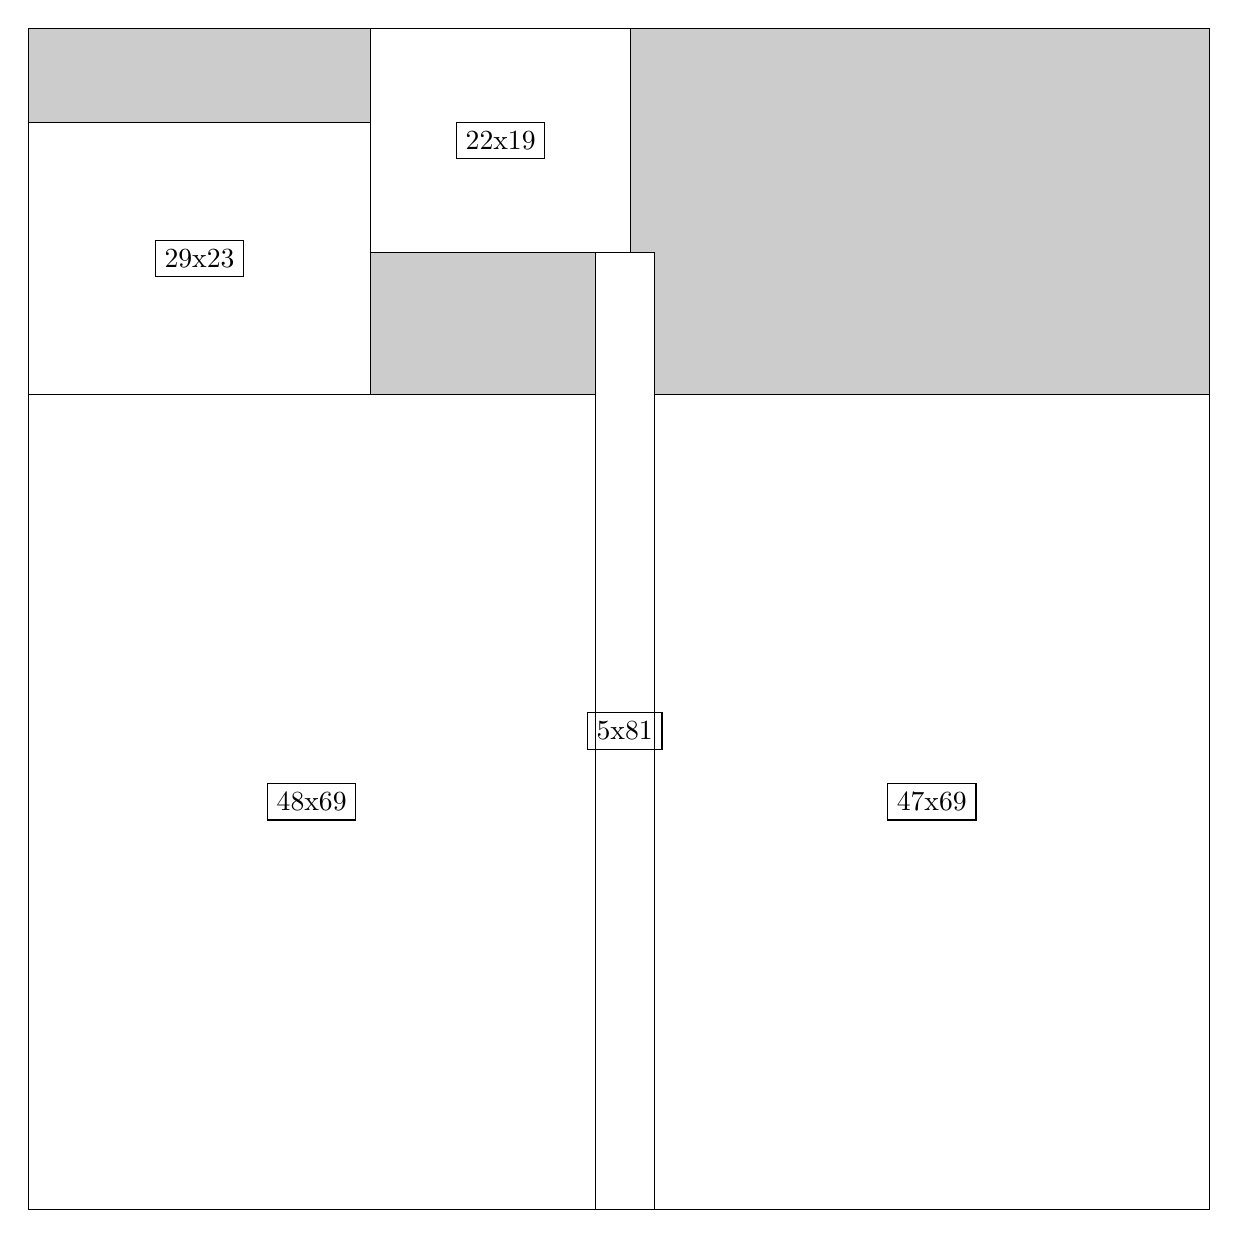
\begin{tikzpicture}[shorten >=1pt,scale=1.0,every node/.style={scale=1.0},->]
\tikzstyle{vertex}=[circle,fill=black!25,minimum size=14pt,inner sep=0pt]
\filldraw[fill=gray!40!white, draw=black] (0,0) rectangle (15.0,15.0);
\foreach \name/\x/\y/\w/\h in {48x69/0.0/0.0/7.199999999999999/10.35,47x69/7.949999999999999/0.0/7.05/10.35,29x23/0.0/10.35/4.35/3.4499999999999997,22x19/4.35/12.15/3.3/2.85,5x81/7.199999999999999/0.0/0.75/12.15}
\filldraw[fill=white!40!white, draw=black] (\x,\y) rectangle node[draw] (\name) {\name} ++(\w,\h);
\end{tikzpicture}


w =48 , h =69 , x =0 , y =0 , v =3312
\par
w =47 , h =69 , x =53 , y =0 , v =3243
\par
w =29 , h =23 , x =0 , y =69 , v =667
\par
w =22 , h =19 , x =29 , y =81 , v =418
\par
w =5 , h =81 , x =48 , y =0 , v =405
\par
\newpage


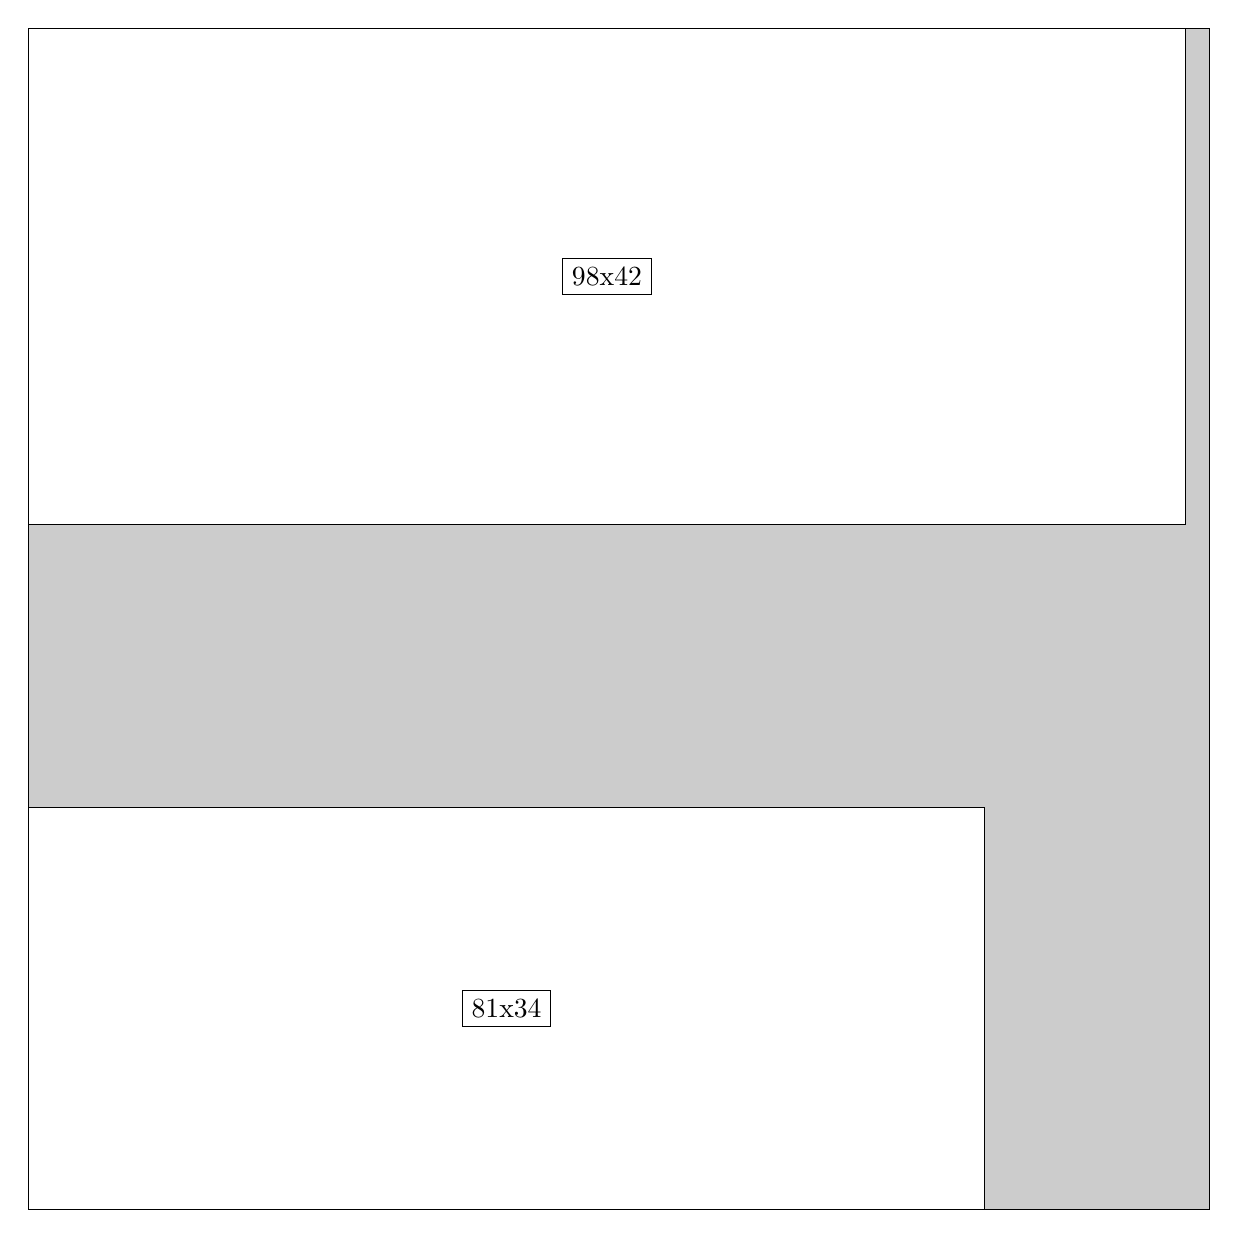
\begin{tikzpicture}[shorten >=1pt,scale=1.0,every node/.style={scale=1.0},->]
\tikzstyle{vertex}=[circle,fill=black!25,minimum size=14pt,inner sep=0pt]
\filldraw[fill=gray!40!white, draw=black] (0,0) rectangle (15.0,15.0);
\foreach \name/\x/\y/\w/\h in {98x42/0.0/8.7/14.7/6.3,81x34/0.0/0.0/12.15/5.1}
\filldraw[fill=white!40!white, draw=black] (\x,\y) rectangle node[draw] (\name) {\name} ++(\w,\h);
\end{tikzpicture}


w =98 , h =42 , x =0 , y =58 , v =4116
\par
w =81 , h =34 , x =0 , y =0 , v =2754
\par
\newpage


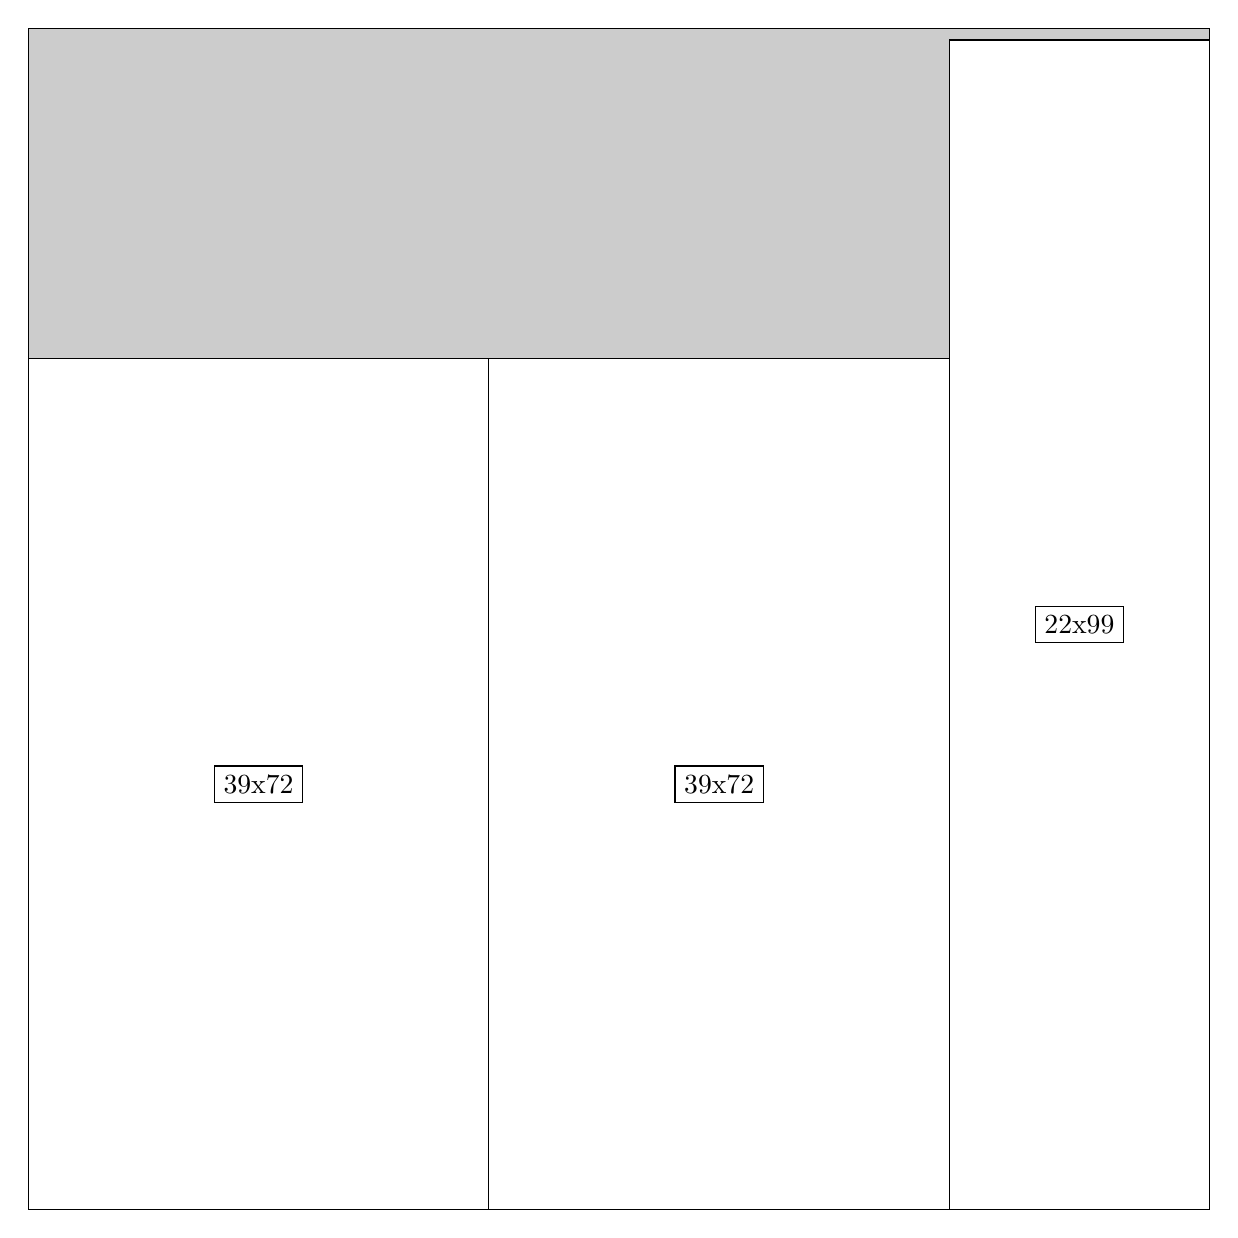
\begin{tikzpicture}[shorten >=1pt,scale=1.0,every node/.style={scale=1.0},->]
\tikzstyle{vertex}=[circle,fill=black!25,minimum size=14pt,inner sep=0pt]
\filldraw[fill=gray!40!white, draw=black] (0,0) rectangle (15.0,15.0);
\foreach \name/\x/\y/\w/\h in {39x72/0.0/0.0/5.85/10.799999999999999,39x72/5.85/0.0/5.85/10.799999999999999,22x99/11.7/0.0/3.3/14.85}
\filldraw[fill=white!40!white, draw=black] (\x,\y) rectangle node[draw] (\name) {\name} ++(\w,\h);
\end{tikzpicture}


w =39 , h =72 , x =0 , y =0 , v =2808
\par
w =39 , h =72 , x =39 , y =0 , v =2808
\par
w =22 , h =99 , x =78 , y =0 , v =2178
\par
\newpage


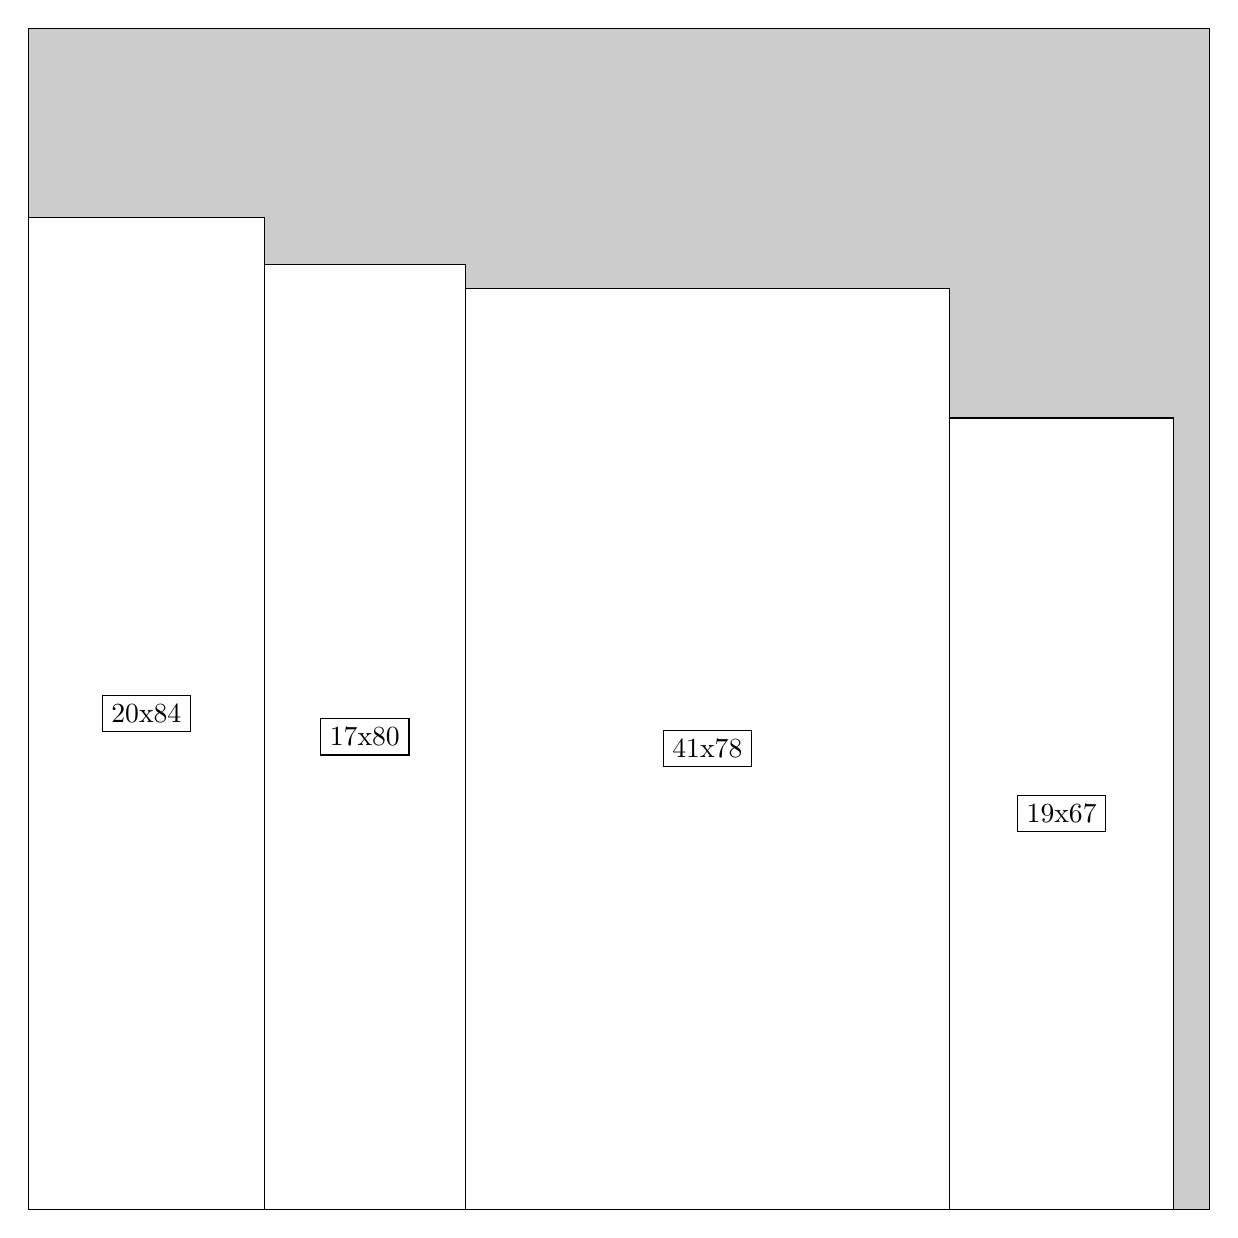
\begin{tikzpicture}[shorten >=1pt,scale=1.0,every node/.style={scale=1.0},->]
\tikzstyle{vertex}=[circle,fill=black!25,minimum size=14pt,inner sep=0pt]
\filldraw[fill=gray!40!white, draw=black] (0,0) rectangle (15.0,15.0);
\foreach \name/\x/\y/\w/\h in {41x78/5.55/0.0/6.1499999999999995/11.7,20x84/0.0/0.0/3.0/12.6,17x80/3.0/0.0/2.55/12.0,19x67/11.7/0.0/2.85/10.049999999999999}
\filldraw[fill=white!40!white, draw=black] (\x,\y) rectangle node[draw] (\name) {\name} ++(\w,\h);
\end{tikzpicture}


w =41 , h =78 , x =37 , y =0 , v =3198
\par
w =20 , h =84 , x =0 , y =0 , v =1680
\par
w =17 , h =80 , x =20 , y =0 , v =1360
\par
w =19 , h =67 , x =78 , y =0 , v =1273
\par
\newpage


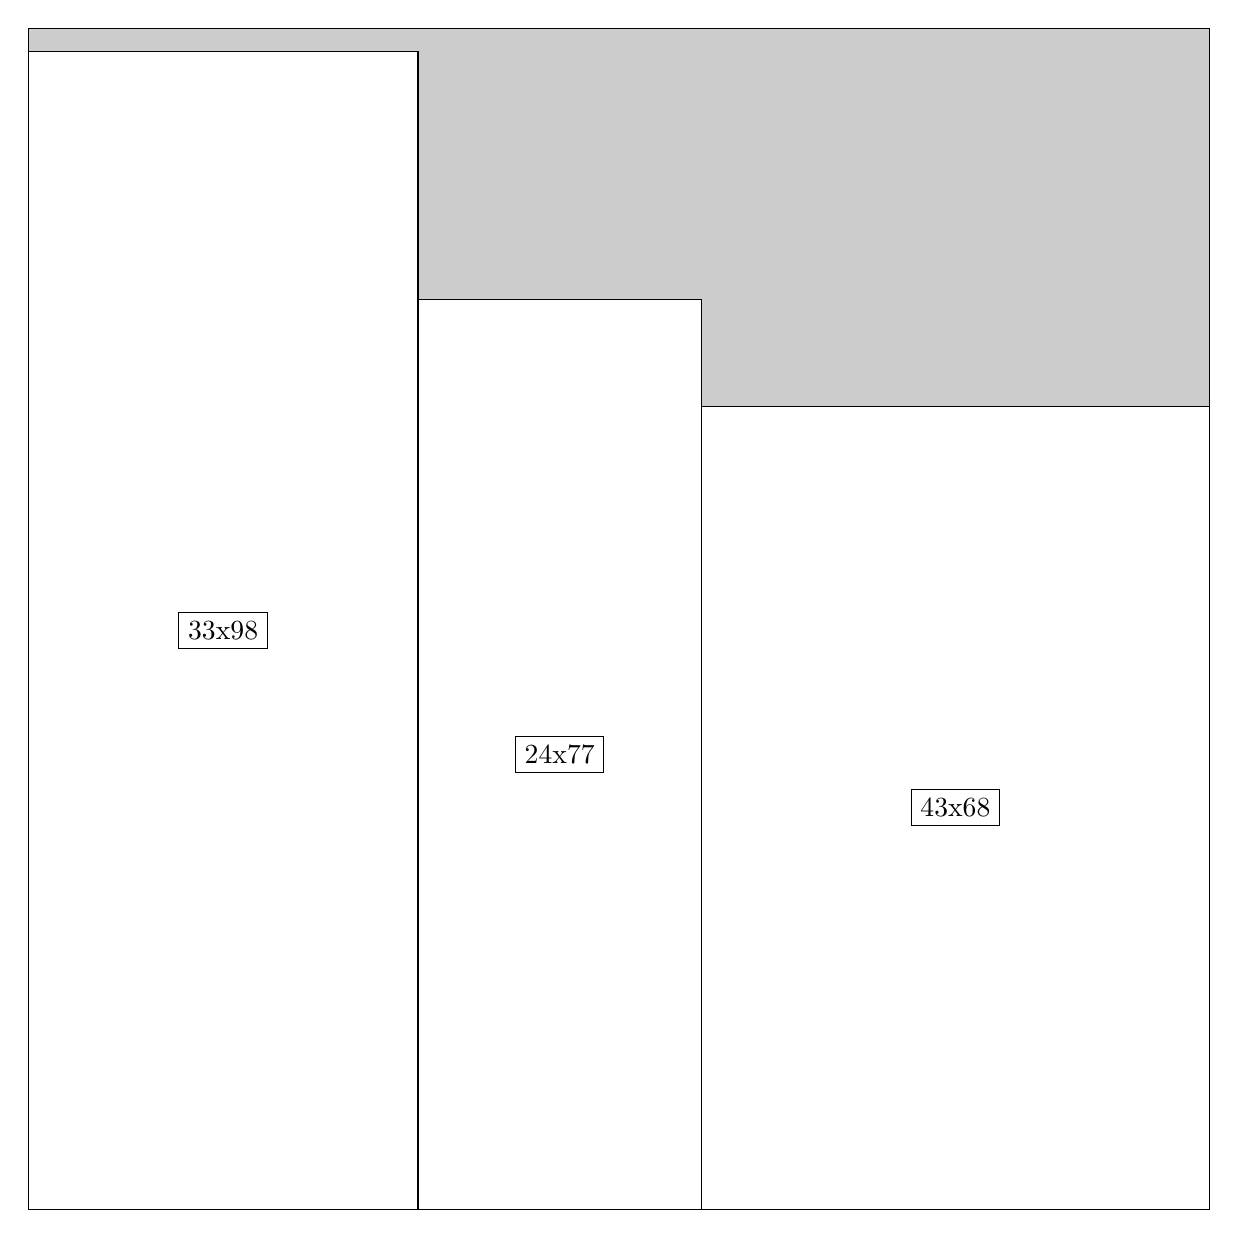
\begin{tikzpicture}[shorten >=1pt,scale=1.0,every node/.style={scale=1.0},->]
\tikzstyle{vertex}=[circle,fill=black!25,minimum size=14pt,inner sep=0pt]
\filldraw[fill=gray!40!white, draw=black] (0,0) rectangle (15.0,15.0);
\foreach \name/\x/\y/\w/\h in {33x98/0.0/0.0/4.95/14.7,43x68/8.549999999999999/0.0/6.45/10.2,24x77/4.95/0.0/3.5999999999999996/11.549999999999999}
\filldraw[fill=white!40!white, draw=black] (\x,\y) rectangle node[draw] (\name) {\name} ++(\w,\h);
\end{tikzpicture}


w =33 , h =98 , x =0 , y =0 , v =3234
\par
w =43 , h =68 , x =57 , y =0 , v =2924
\par
w =24 , h =77 , x =33 , y =0 , v =1848
\par
\newpage


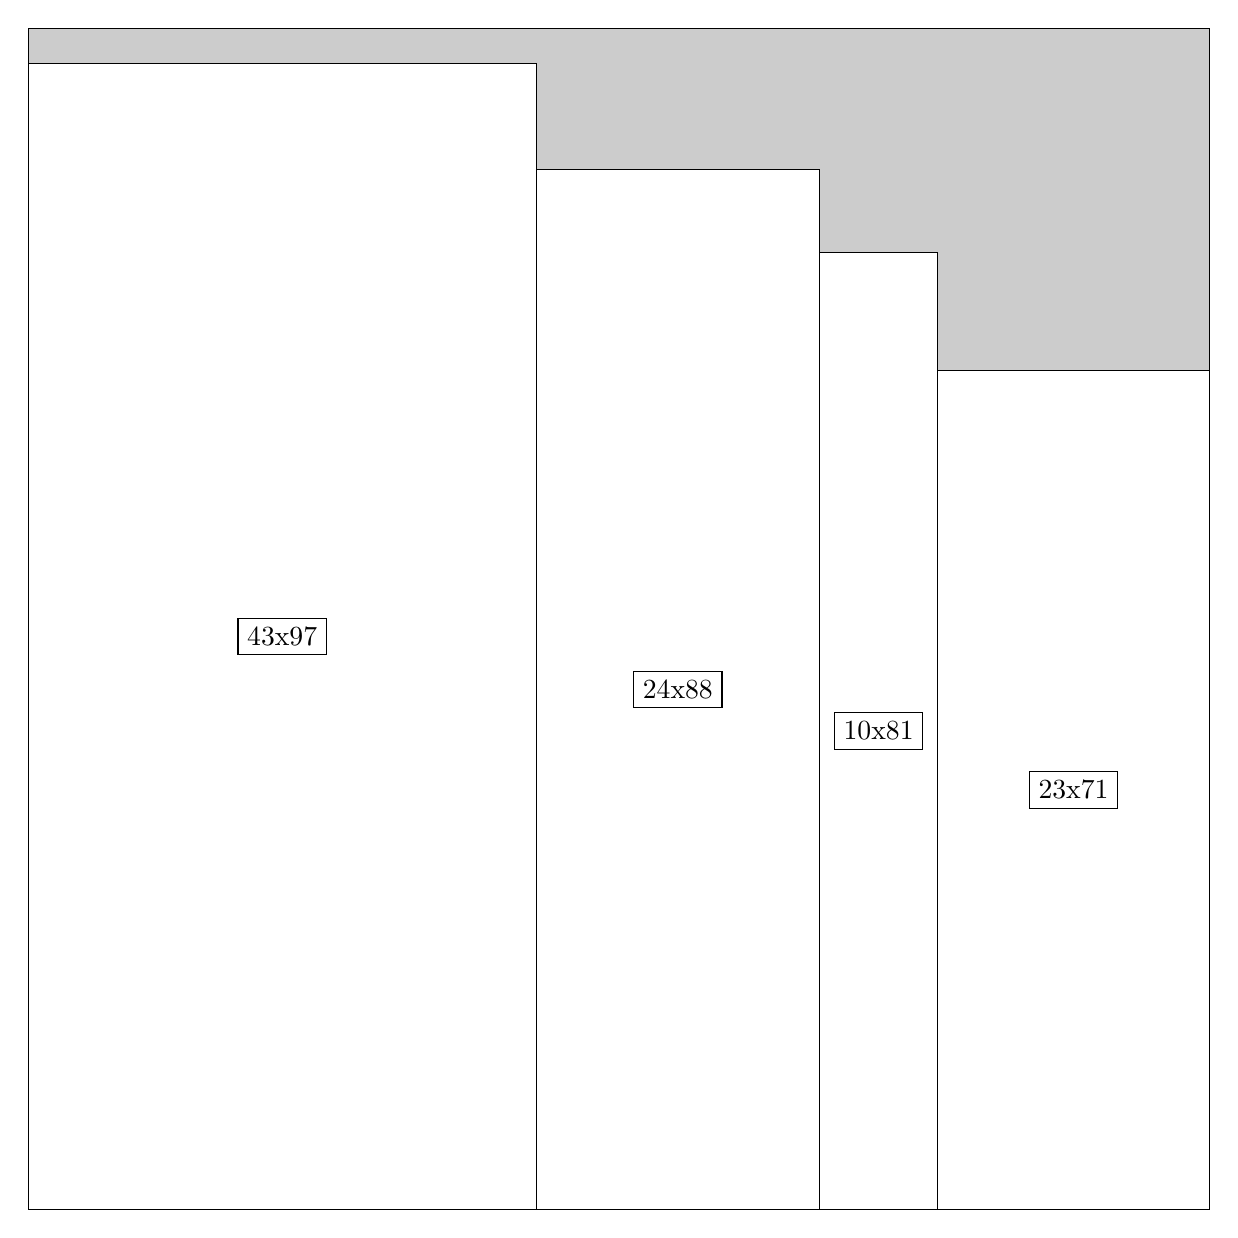
\begin{tikzpicture}[shorten >=1pt,scale=1.0,every node/.style={scale=1.0},->]
\tikzstyle{vertex}=[circle,fill=black!25,minimum size=14pt,inner sep=0pt]
\filldraw[fill=gray!40!white, draw=black] (0,0) rectangle (15.0,15.0);
\foreach \name/\x/\y/\w/\h in {43x97/0.0/0.0/6.45/14.549999999999999,24x88/6.45/0.0/3.5999999999999996/13.2,23x71/11.549999999999999/0.0/3.4499999999999997/10.65,10x81/10.049999999999999/0.0/1.5/12.15}
\filldraw[fill=white!40!white, draw=black] (\x,\y) rectangle node[draw] (\name) {\name} ++(\w,\h);
\end{tikzpicture}


w =43 , h =97 , x =0 , y =0 , v =4171
\par
w =24 , h =88 , x =43 , y =0 , v =2112
\par
w =23 , h =71 , x =77 , y =0 , v =1633
\par
w =10 , h =81 , x =67 , y =0 , v =810
\par
\newpage


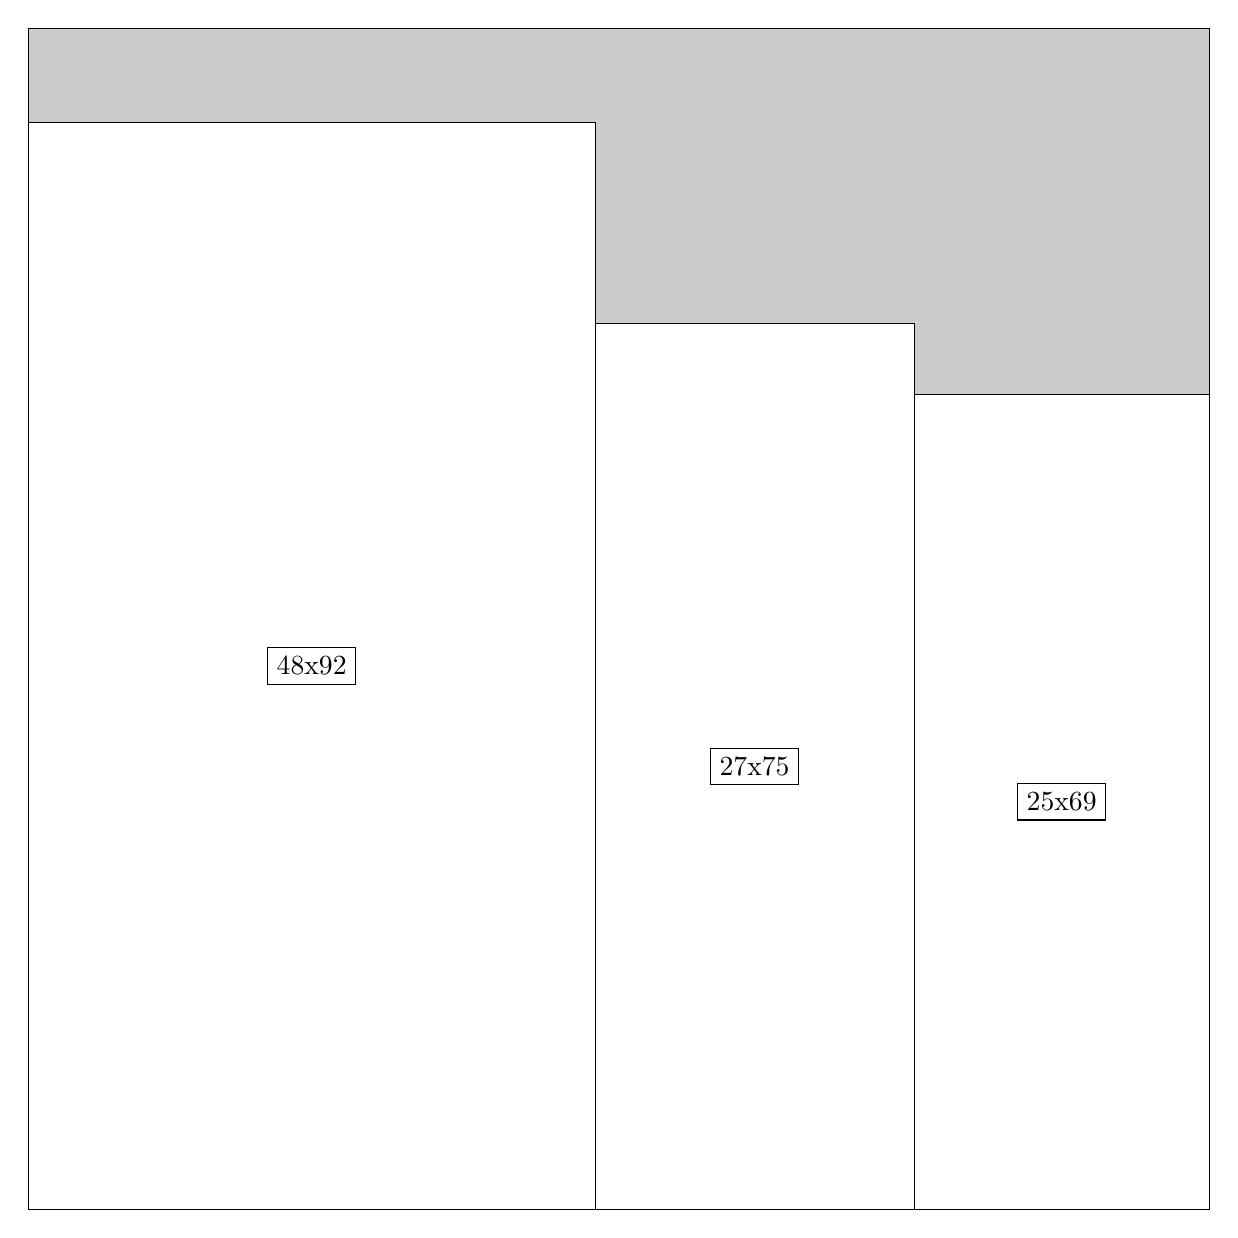
\begin{tikzpicture}[shorten >=1pt,scale=1.0,every node/.style={scale=1.0},->]
\tikzstyle{vertex}=[circle,fill=black!25,minimum size=14pt,inner sep=0pt]
\filldraw[fill=gray!40!white, draw=black] (0,0) rectangle (15.0,15.0);
\foreach \name/\x/\y/\w/\h in {48x92/0.0/0.0/7.199999999999999/13.799999999999999,27x75/7.199999999999999/0.0/4.05/11.25,25x69/11.25/0.0/3.75/10.35}
\filldraw[fill=white!40!white, draw=black] (\x,\y) rectangle node[draw] (\name) {\name} ++(\w,\h);
\end{tikzpicture}


w =48 , h =92 , x =0 , y =0 , v =4416
\par
w =27 , h =75 , x =48 , y =0 , v =2025
\par
w =25 , h =69 , x =75 , y =0 , v =1725
\par
\newpage


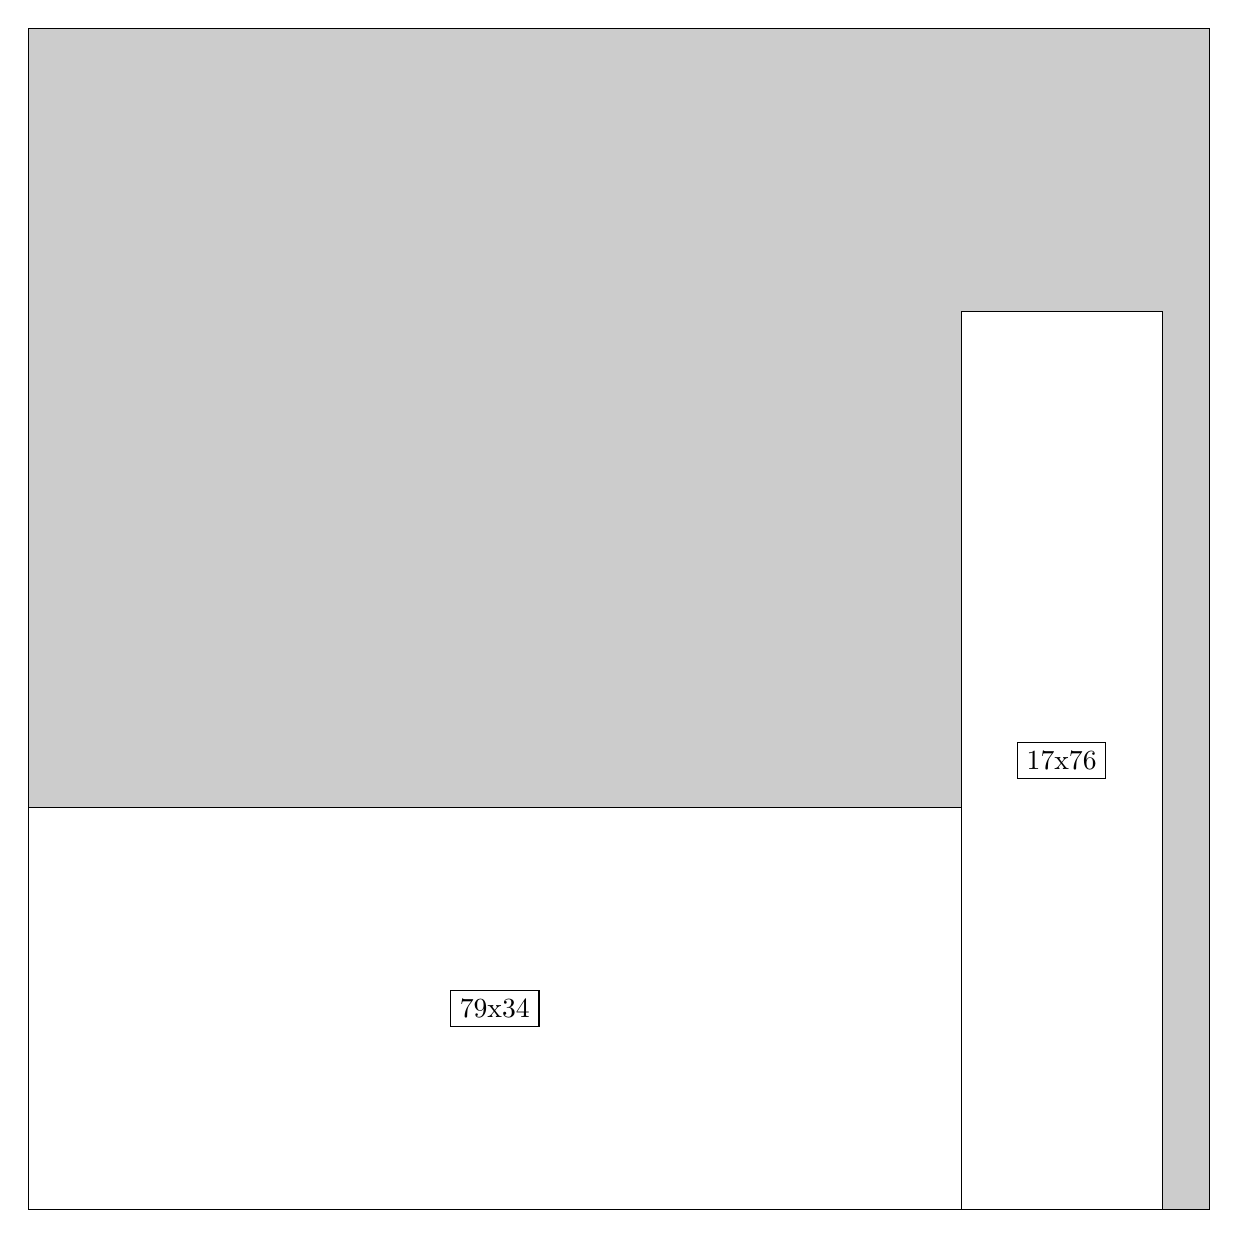
\begin{tikzpicture}[shorten >=1pt,scale=1.0,every node/.style={scale=1.0},->]
\tikzstyle{vertex}=[circle,fill=black!25,minimum size=14pt,inner sep=0pt]
\filldraw[fill=gray!40!white, draw=black] (0,0) rectangle (15.0,15.0);
\foreach \name/\x/\y/\w/\h in {79x34/0.0/0.0/11.85/5.1,17x76/11.85/0.0/2.55/11.4}
\filldraw[fill=white!40!white, draw=black] (\x,\y) rectangle node[draw] (\name) {\name} ++(\w,\h);
\end{tikzpicture}


w =79 , h =34 , x =0 , y =0 , v =2686
\par
w =17 , h =76 , x =79 , y =0 , v =1292
\par
\newpage


\end{document}